\documentclass[times,twocolumn]{aastex62}

\hypersetup{colorlinks=false}

%%%% Define Acronyms
\usepackage{acronym}
%
\newacro{MBH}{massive black hole}
\newacroplural{MBH}[MBHs]{massive black holes}
\newcommand{\MBH}{\ac{MBH}}
\newcommand{\MBHs}{\acp{MBH}}

%%%% Math %%%%
\usepackage{commath}
\usepackage{bm}
\usepackage{mathtools}


%%%% Show Equations labels %%%%
% \usepackage[notcite,notref]{showkeys}
% \renewcommand*\showkeyslabelformat[1]{\normalfont\tiny\ttfamily#1}
%%%%%%



% Defs


% Roman
\newcommand{\rd}{\mathrm{d}}
\newcommand{\re}{\mathrm{e}}
\newcommand{\ri}{\mathrm{i}}


% Int
\usepackage{xargs}
\newcommandx\dint[2][usedefault, addprefix=\global, 1=, 2=]{\!\!\int_{#1}^{#2}\!\! \rd}


%comments
\usepackage{soul} % To allow for the use of \hl.

% Equations
\newcommand\eq{equation}
\newcommand\eqs{equations}
\newcommand\Eq{Equation}
\newcommand\Eqs{Equations}


%\submitjournal{ApJL}


\shorttitle{short title}
\shortauthors{Bar-Or and \dots}

\begin{document}

\title{Title}

\author{Ben Bar-Or}
\affiliation{Institute for Advanced Study, Princeton, NJ, USA}

\author{\dots}
\affiliation{Institute for Advanced Study, Princeton, NJ, USA}

\keywords{gravitation --- black hole physics --- galaxies: nuclei}

\begin{abstract}
  abstract
\end{abstract}


%%%%%%%%%%%%%%%%%%%%
\section{Introduction}
Figure~\ref{fig:example}

\cite{Bar-Or+2016} 

\begin{figure}[h]
  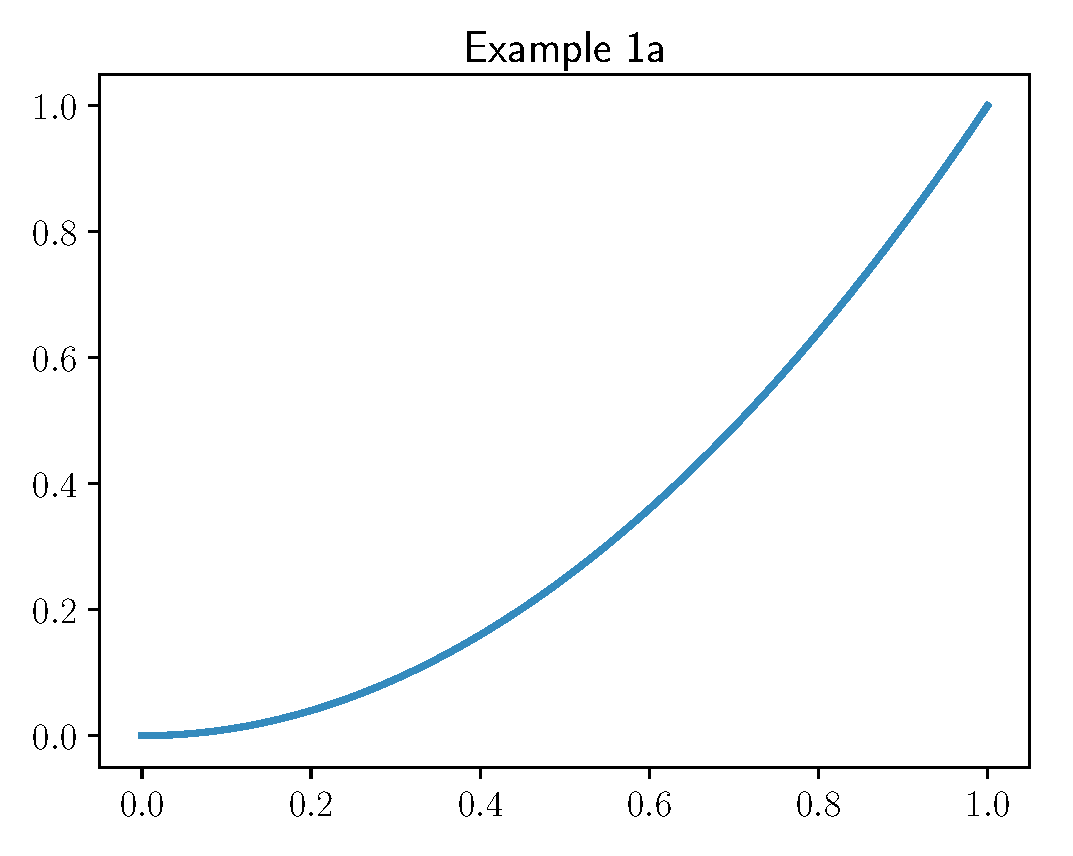
\includegraphics[width=0.48\textwidth]{figures/example_1a}
  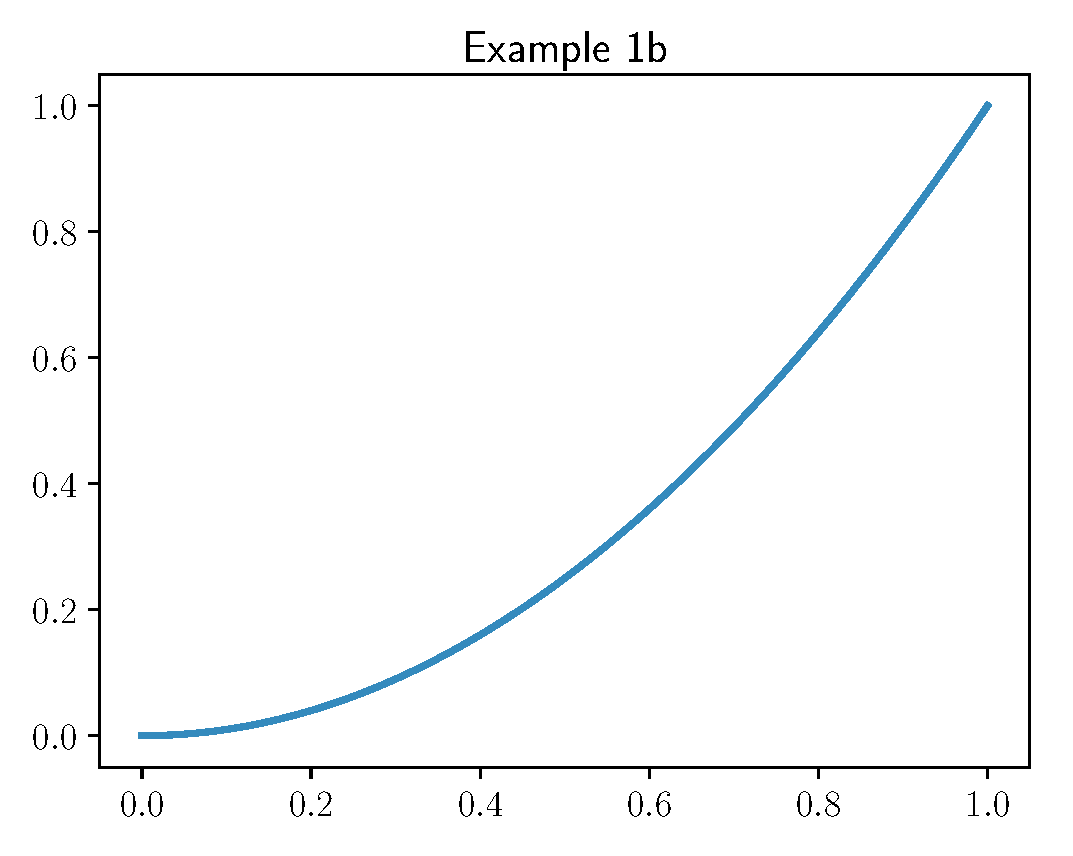
\includegraphics[width=0.48\textwidth]{figures/example_1b}
  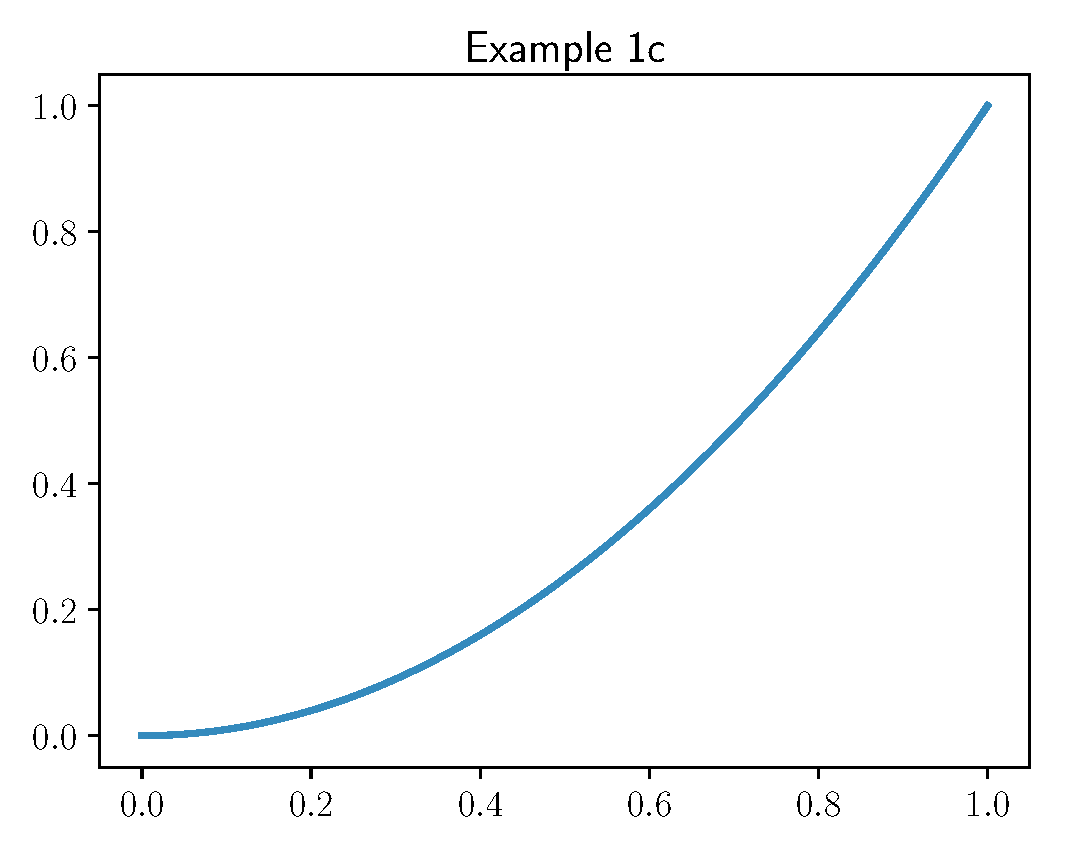
\includegraphics[width=0.48\textwidth]{figures/example_1c}
\caption{\label{fig:example}}
\end{figure}

\begin{figure}[h]
\plotone{figures/example_2}
\caption{\label{fig:example}}
\end{figure}



%%%%%%%%%%%%%%%%%%%%
\acknowledgments\

We thank \dots

%%%%%%%%%%%%%%%%%%%%


%%%%%%%%%%%%%%%%%%%%
\bibliographystyle{apj}
\bibliography{main}
%%%%%%%%%%%%%%%%%%%%



\end{document}
